\chapter{More on certificate authentication}
\index{Certificate authentication}
\label{certificate}

\section{The X.509\index{X.509 certificates} trust model}
\label{x509:trust}

The X.509 protocols rely on a hierarchical trust model. In this trust model
Certification Authorities (CAs) are used to certify entities.
Usually more than one certification authorities exist, and certification
authorities may certify other authorities to issue certificates as well,
following a hierarchical model. 
One needs to trust one or more CAs for his secure
communications. In that case only the certificates issued by the trusted
authorities are acceptable. See figure \ref{fig:x509-1} for a typical example.

\begin{figure}[hbtp]
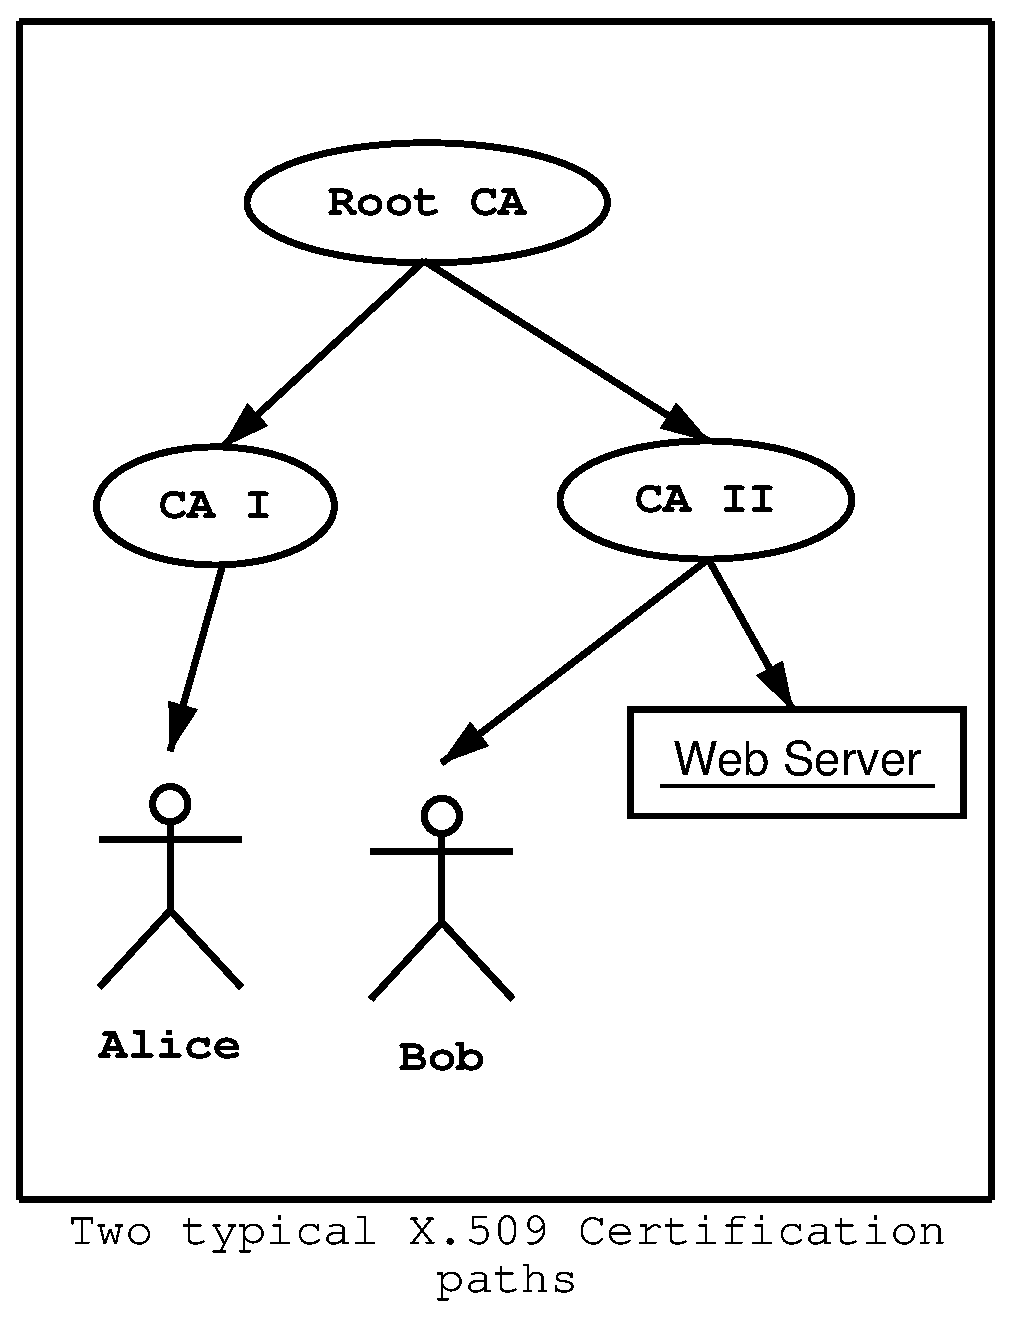
\includegraphics[height=9.5cm,width=9cm]{x509-1}
\label{fig:x509-1}
\end{figure}

\par The use of X.509 certificates requires some functions which will 
assist in parsing them. \gnutls{} includes functions which extract 
parameters from given X.509 certificates. Some of them are:
\begin{itemize}
\item \printfunc{gnutls_x509_extract_certificate_dn}{gnutls\_x509\_extract\_certificate\_dn}
\item \printfunc{gnutls_x509_extract_certificate_serial}{gnutls\_x509\_extract\_certificate\_serial}
\item \printfunc{gnutls_x509_extract_certificate_subject_alt_name}{gnutls\_x509\_extract\_certificate\_subject\_alt\_name}
\end{itemize}

Given the complexity of the X.509 protocols we do not expect these limited 
functions to cover every need. Thus a function which converts X.509 DER certificates
to an XML form is provided. See appendix \ref{ap:xml} on page \pageref{ap:xml} for
more information.


\par
Verifying certificate\index{Verifying certificate paths} paths is important 
in X.509 authentication. For this purpose you should use functions like
\printfunc{gnutls_x509_verify_certificate}{gnutls\_x509\_verify\_certificate}.
A more generic one is also provided and can be used with all
of the certificate authentication methods, but is limited to a session. See the
\printfunc{gnutls_certificate_verify_peers}{gnutls\_certificate\_verify\_peers}
function. The above functions verify if the given certificate path leads
to a trusted CA certificate. You should also verify if the certificate's
owner is the one you expect. See section \ref{ex:rfc2818} on page \pageref{ex:rfc2818},
for an example.

\par
Client certificate authentication\index{Certificate authentication!Client} is 
optional in \tls{}. A server may request a certificate from the client -- using the
\printfunc{gnutls_certificate_server_set_request}{gnutls\_certificate\_server\_set\_request}
function. If a certificate is to be requested by the client, at the handshake 
procedure, the server will send an extra packet,
than contains a list of acceptable certificate signers, and indicates the
request of a certificate. The client may then send a certificate, signed
by one of the server's acceptable signers. In \gnutls{} the server's acceptable
signers list is constructed using the trusted CA certificates in the
credentials structure.

\par
Note that \gnutls{} is not a generic purpose X.509 toolkit\footnote{Aegypten is such a toolkit. See 
\htmladdnormallink{http://www.gnupg.org/aegypten/}{http://www.gnupg.org/aegypten/}}. 
\gnutls{} only includes the required,
in order to use the TLS cipher suites which depend on X.509 certificates.


\section{The OpenPGP\index{OpenPGP!Keys} trust model}
\label{pgp:trust}

The OpenPGP key authentication relies on a distributed trust model, called
the "web of trust". The "web of trust" uses a decentralized system of 
trusted introducers, which are the same as a CA. OpenPGP allows anyone to 
sign anyone's else public key. When Alice signs Bob's key, she is introducing 
Bob's key to anyone who trusts Alice. If someone trusts Alice to introduce
keys, then Alice is a trusted introducer in the mind of that observer.

\begin{figure}[hbtp]
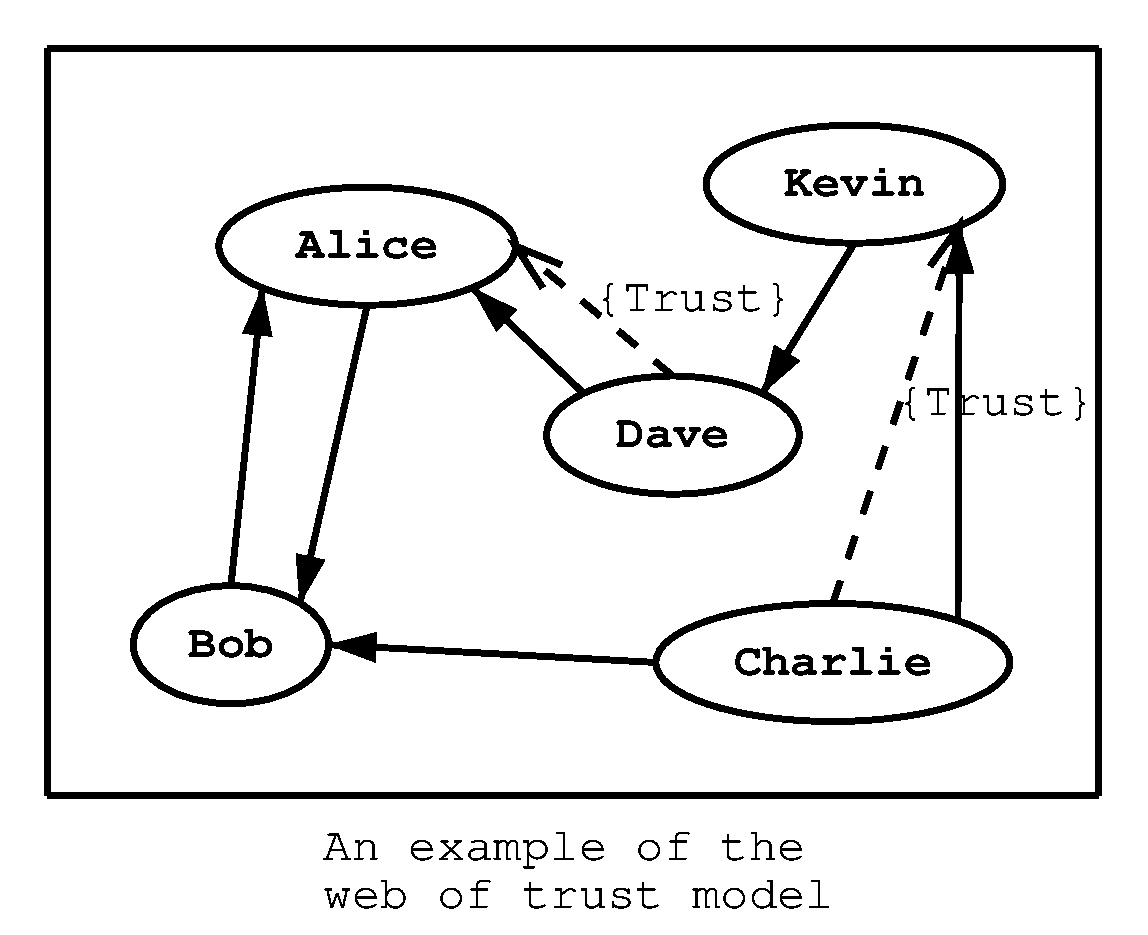
\includegraphics[height=9cm,width=11cm]{pgp-fig1}
\label{fig:pgp1}
\end{figure}

For example: If David trusts Alice to be an introducer, and Alice signed
Bob's key, Dave also trusts Bob's key to be the real one.

There are some key points that are important in that model. In the example
Alice has to sign Bob's key, only if she is sure that the key belongs
to Bob. Otherwise she may also make Dave falsely believe that this
is Bob's key. Dave has also the responsibility to know who to trust.
This model is similar to real life relations.

Just see how Charlie behaves in the previous example. Although he has 
signed Bob's key - because he knows, somehow, that it belongs to Bob - 
he does not trust Bob to be an introducer. Charlie decided to trust only 
Kevin, for some reason. A reason could be that Bob is lazy enough, and 
signs other people's keys without being sure that they belong to the 
actual owner.

\subsection{Verifying an OpenPGP key}
First we've to differentiate between ownertrust and validity. Sometimes trust
and validity is used as a synonym but this is not correct.
\par
The ownertrust describes how trustworthy the signature of a special
key owner is. Even if we've three or more signatures to make a key valid,
it's possible that we don't trust the owner at all and thus we don't trust 
the signature he made. There are different ownertrust levels:
\begin{enumerate}
\item Don't know
\item I do NOT trust
\item I trust marginally
\item I trust fully
\item I trust ultimately.
\end{enumerate}

For example we need three marginally trusted signature to make a key
valid or one full trusted signature. The ultimate trust is only used
when we are the owner of a key and we also have the secret key.
In the case we don't trust the owner, those signatures are skipped
for the web of trust calculation.
\par
All checks in GnuTLS are done in \printfunc{gnutls_openpgp_verify_key}{gnutls\_openpgp\_verify\_key}. 
If a trust database is available, this is the file which contains all information about the
key owner (ownertrust), additional checks are performed.
\\
First we get the trustdb entry to see if the key is not disabled because
those keys shouldn't be used at all. Another possible case is that we
don't trust the key, which means we don't need to perform further checks.
\par
If the ownertrust is at least marginal we continue to check all signatures
the key contains to get the validity of the key. It is likely that the
public keyring does not contain all needed keys to check all signatures.
When a signature could not be checked due to a missing key, the function 
tries the next signature. When NO public key is available, the function
checks at least the self signature which must be valid in any case because
it was created by the key itself.
\\
Validity means if the signatures on the key are valid and the key was not 
changed by somebody or corrupted during transport.

